% This tex file is available under a
% Creative Commons Attribution-Share Alike license (CC BY-SA 2.0).
% http://creativecommons.org/licenses/by-sa/2.0/
% Copyright © 2013 Rodrigo Hausen
\documentclass{beamer}
\usepackage[utf8]{inputenc}
\usepackage{lmodern}
\usepackage[T1]{fontenc}
\usepackage[portuguese,brazil]{babel}
\usepackage{url}
\usepackage{listings}
\usepackage{color}
\usepackage{textcomp}
\usepackage{pdfpages}
\usepackage{fancyvrb}
\usepackage{enumerate}
\usepackage{icomma} % para vírgula decimal / decimal comma
\definecolor{listinggray}{gray}{0.9}
\definecolor{lbcolor}{rgb}{0.9,0.9,0.9}
\definecolor{mediumgray}{rgb}{0.6,0.6,0.6}
\lstset{
    backgroundcolor=\color{lbcolor},
    tabsize=4,
    rulecolor=,
    basicstyle=\scriptsize,
    upquote=true,
    aboveskip={1.5\baselineskip},
    columns=fixed,
    showstringspaces=false,
    extendedchars=true,
    breaklines=true,
    prebreak = \raisebox{0ex}[0ex][0ex]{\ensuremath{\hookleftarrow}},
    frame=single,
    showtabs=false,
    showspaces=false,
    showstringspaces=false,
    identifierstyle=\ttfamily,
    keywordstyle=\color[rgb]{0,0,1},
    commentstyle=\color[rgb]{0.133,0.545,0.133},
    stringstyle=\color[rgb]{0.627,0.126,0.941},
}

\definecolor{pinegreen}{RGB}{0,139,114}
\definecolor{pgr}{RGB}{0,139,114}

\definecolor{aquamarine}{RGB}{0,181,190}
\definecolor{aqm}{RGB}{0,181,190}

\definecolor{skyblue}{RGB}{100,227,251}
\definecolor{skb}{RGB}{100,227,251}

\newcommand{\comment}[1]{{\color{structure.fg!70!white}\footnotesize #1}}

\newcommand{\WD}[1]{\fbox{#1}\hspace{-0.5pt}}

\newcommand{\FWD}[1]{%
\fbox{%
\vbox to 10pt{\vfil%
\hbox to 0.8cm{\hfill#1\hfill}%
\vfil}%
}\hspace{-0.5pt}%
}

\def\A{\texttt{A}}
\def\B{\texttt{B}}
\def\C{\texttt{C}}
\def\D{\texttt{D}}
\def\E{\texttt{E}}
\def\F{\texttt{F}}

\usetheme{Boadilla}
%\usetheme{umbc2}
\usefonttheme{structuresmallcapsserif}
\usecolortheme{seahorse}

\title{Aula 4: Álgebra booleana}
\subtitle{Circuitos Digitais}
\author{Rodrigo Hausen}
\institute{CMCC -- UFABC} 
\date{01 de fevereiro de 2013}

\begin{document}

\begin{frame}
\maketitle

\vspace{-1cm}

\begin{center}
\url{http://compscinet.org/circuitos}
\end{center}

\end{frame}

%%%%%%%%%%%%%%%%%%%%%%%%%%%%%%%

\begin{frame}
 \frametitle{Uma álgebra diferente}

\begin{minipage}{0.62\textwidth}
 \textbf{Álgebra booleana} [Boole, 1854]
 \begin{itemize}
 \item Álgebra onde há apenas dois valores válidos: \textbf{falso} e
\textbf{verdadeiro}.
 \pause
 \item Também denotados:
 \begin{itemize}
   \item \textbf{F} e \textbf{V};
   \pause
   \item \textbf{false} e \textbf{true} (ou \textbf{F} e \textbf{T});
   \pause
   \item \textbf{desligado} e \textbf{ligado};
   \pause
   \item \textbf{nível baixo} e \textbf{nível alto} de um sinal;
   \pause
   \item \textbf{0} e \textbf{1}, etc.
 \end{itemize}
\pause
 \item Variável booleana: pode assumir um dos dois valores booleanos válidos.
    \begin{itemize}
        \item Geralmente denotada por uma letra maiúscula: $A$, $B$, $C$, $X$, $Y$, $Z$, \ldots
    \end{itemize}
 \end{itemize}
\end{minipage}
%
\pause
\begin{minipage}{0.37\textwidth}
\hfill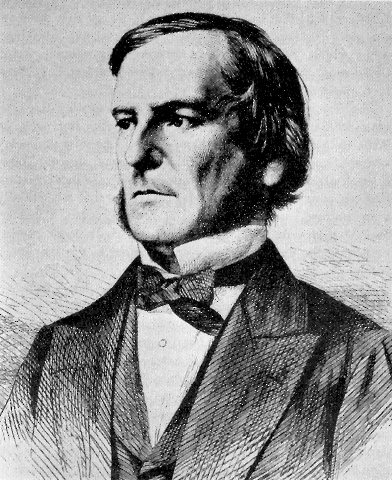
\includegraphics[width=0.95\textwidth]{images/georgeboole}%
\hfill\phantom{.}\\
\footnotesize{\color{gray}George Boole (1815--1864). Ma\-te\-má\-ti\-co e
filósofo inglês, ``pai'' da lógica digital moderna.}\\\comment{\tiny{\href{http://pt.wikipedia.org/wiki/George_Boole}{http://pt.wikipedia.org/wiki/George\_Boole}}}
\end{minipage}

\end{frame}

\begin{frame}
\frametitle{Operações básicas}

\def\spc{ \hspace{4ex} }

As operações básicas da álgebra booleana são:
\begin{itemize}
 \item \emph{conjunção} ou \emph{multiplicação booleana}:\\
       $X \textbf{ e } Y$ \spc $X \textbf{ and } Y$ \spc $X \wedge Y$ \spc
       \fcolorbox{skb}{skb}{$X \cdot Y$}
\pause
 \item \emph{disjunção} ou \emph{produto booleano}:\\
       $X \textbf{ ou } Y$ \spc $X \textbf{ or } Y$ \spc $X \vee Y$ \spc
       \fcolorbox{skb}{skb}{$X + Y$}
\pause
 \item \emph{negação} ou \emph{complemento}:\\
       $\textbf{não } X$ \spc $\textbf{not }X$ \spc $\sim\!X$ \spc
       $\lnot X$ \spc \fcolorbox{skb}{skb}{$\overline{X}$}
\end{itemize}
\pause

\vspace{16pt}

Em Java, respectivamente: $X \, \&\& \, Y$,
$X \, || \, Y$, $ !X $
\end{frame}

%%%%%%%%%%%%%%%%%%%%%%%%%%%%%%%

\begin{frame}
 \frametitle{Tabuadas da álgebra booleana}

 Assim como na álgebra comum, o resultado de uma operação booleana é obtido
através de uma tabuada. Na álgebra booleana, as tabuadas são chamadas
\textbf{tabelas verdade}.\\[12pt]

\pause

\hspace{4ex}
%
\begin{minipage}{16ex}
\centering
Tabela verdade da conjunção (\textbf{e})\\[6pt]
\begin{tabular}{cc|c}
 $x$ & $y$ & $x \cdot y$ \\
\hline
 $F$ & $F$ & $F$ \\
 $F$ & $V$ & $F$ \\
 $V$ & $F$ & $F$ \\
 $V$ & $V$ & $V$
\end{tabular}
\end{minipage}
%
\hspace{3ex}
%
\begin{minipage}{18ex}
\centering
Tabela verdade da disjunção  (\textbf{ou})\\[6pt]
\begin{tabular}{cc|c}
 $x$ & $y$ & $x + y$ \\
\hline
 $F$ & $F$ & $F$ \\
 $F$ & $V$ & $V$ \\
 $V$ & $F$ & $V$ \\
 $V$ & $V$ & $V$
\end{tabular}
\end{minipage}
%
\hspace{3ex}
%
\begin{minipage}{18ex}
\centering
Tabela verdade da negação  (\textbf{não})\\[12pt]
\begin{tabular}{c|c}
 $x$ & $\overline{x}$ \\
\hline
 $F$ & $V$ \\
 $V$ & $F$
\end{tabular}
\end{minipage}

\pause

\begin{itemize}
 \item Conjunção (oper. \textbf{e}): resultado
verdadeiro apenas se $x$ \textbf{e} $y$ forem verdadeiros.
\pause
 \item Disjunção (oper. \textbf{ou}): resultado
verdadeiro apenas se $x$ \textbf{ou} $y$ forem verdadeiros.
\pause
 \item Negação: resultado só será verdadeiro se $x$ \textbf{não} for
verdadeiro.
\end{itemize}

\end{frame}

%%%%%%%%%%%%%%%%%%%%%%%%%%%%%%%

\begin{frame}
 \frametitle{Tabelas verdade com valores $0$ e $1$}
Equivalências: F = 0, V = 1\\[6pt]

\hspace{4ex}
%
\begin{minipage}{16ex}
\centering
Tabela verdade da conjunção (\textbf{e})\\[6pt]
\begin{tabular}{cc|c}
 $x$ & $y$ & $x \cdot y$ \\
\hline
 $F$ & $F$ & $F$ \\
 $F$ & $V$ & $F$ \\
 $V$ & $F$ & $F$ \\
 $V$ & $V$ & $V$
\end{tabular}
\end{minipage}
%
\hspace{3ex}
%
\begin{minipage}{18ex}
\centering
Tabela verdade da disjunção  (\textbf{ou})\\[6pt]
\begin{tabular}{cc|c}
 $x$ & $y$ & $x + y$ \\
\hline
 $F$ & $F$ & $F$ \\
 $F$ & $V$ & $V$ \\
 $V$ & $F$ & $V$ \\
 $V$ & $V$ & $V$
\end{tabular}
\end{minipage}
%
\hspace{3ex}
%
\begin{minipage}{18ex}
\centering
Tabela verdade da negação  (\textbf{não})\\[12pt]
\begin{tabular}{c|c}
 $x$ & $\overline{x}$ \\
\hline
 $F$ & $V$ \\
 $V$ & $F$
\end{tabular}
\end{minipage}

\pause

\vspace{6pt}

\hspace{4ex}
%
\begin{minipage}{16ex}
\centering
Tabela verdade da conjunção (\textbf{e})\\[6pt]
\begin{tabular}{cc|c}
 $x$ & $y$ & $x \cdot y$ \\
\hline
 $0$ & $0$ & $0$ \\
 $0$ & $1$ & $0$ \\
 $1$ & $0$ & $0$ \\
 $1$ & $1$ & $1$
\end{tabular}
\end{minipage}
%
\hspace{3ex}
%
\begin{minipage}{18ex}
\centering
Tabela verdade da disjunção  (\textbf{ou})\\[6pt]
\begin{tabular}{cc|c}
 $x$ & $y$ & $x + y$ \\
\hline
 $0$ & $0$ & $0$ \\
 $0$ & $1$ & $1$ \\
 $1$ & $0$ & $1$ \\
 $1$ & $1$ & $1$
\end{tabular}
\end{minipage}
%
\hspace{3ex}
%
\begin{minipage}{18ex}
\centering
Tabela verdade da negação  (\textbf{não})\\[12pt]
\begin{tabular}{c|c}
 $x$ & $\overline{x}$ \\
\hline
 $1$ & $0$ \\
 $0$ & $1$
\end{tabular}
\end{minipage}

\end{frame}

%%%%%%%%%%%%%%%%%%%%%%%%%%%%%%%%%%%%%%%%%%%%%%%%%

\begin{frame}
 \frametitle{Tabelas verdade com valores $0$ e $1$}

\addtolength\fboxrule{1pt}
\begin{center}
\fcolorbox{red}{white}{\begin{minipage}{0.9\textwidth}
\begin{center}
\textbf{Cuidado!} Não confunda tabelas verdade com tabuadas
da\\[6pt] aritmética na base 2.
\end{center}
\end{minipage}}
\end{center}

\addtolength\fboxrule{-1pt}

\vspace{6pt}

\hspace{4ex}
%
\begin{minipage}{16ex}
\centering
Tabela verdade da conjunção (\textbf{e})\\[6pt]
\begin{tabular}{cc|c}
 $x$ & $y$ & $x \cdot y$ \\
\hline
 $0$ & $0$ & $0$ \\
 $0$ & $1$ & $0$ \\
 $1$ & $0$ & $0$ \\
 $1$ & $1$ & $1$
\end{tabular}
\end{minipage}
%
\hspace{3ex}
%
\begin{minipage}{18ex}
\centering
Tabela verdade da disjunção  (\textbf{ou})\\[6pt]
\begin{tabular}{cc|c}
 $x$ & $y$ & $x + y$ \\
\hline
 $0$ & $0$ & $0$ \\
 $0$ & $1$ & $1$ \\
 $1$ & $0$ & $1$ \\
 \fcolorbox{skb}{skb}{\phantom{X}\hspace{7.7ex}}\hspace{-11ex} $1$ & $1$ & $1$
\end{tabular}
\end{minipage}
%
\hspace{3ex}
%
\begin{minipage}{18ex}
\centering
Tabela verdade da negação  (\textbf{não})\\[12pt]
\begin{tabular}{c|c}
 $x$ & $\overline{x}$ \\
\hline
 $1$ & $0$ \\
 $0$ & $1$
\end{tabular}
\end{minipage}

\pause

\vspace{12pt}

A partir de agora, daremos preferência a representar os valores lógicos por
0 e 1 (exceto quando for mais claro representar por F e V).

\end{frame}

%%%%%%%%%%%%%%%%%%%%%%%%%%%%%%%%%%%%%%%%%%%%%%%%%

\begin{frame}
 \frametitle{Expressões lógicas}

\begin{itemize}
 \item Como na álgebra comum, podemos combinar as operações, formando
\textbf{expressões lógicas}.
 \item O resultado de uma expressão lógica pode ser calculado aplicando-se cada
operação lógica, consultando-se as tabelas verdade correspondentes.
 \item Para indicar a ordem de aplicação das operações, usam-se parênteses como
na álgebra comum.
 \item Ex 1.: calcule o resultado da expressão abaixo:\\
$\overline{1} + (0 \cdot 1) \pause = \pause 0 \pause + \pause \only<5>{( 0 \cdot
1 )} \only<6>{( 0 )} \only<7->{0} \pause\pause\pause = \pause
\fcolorbox{skb}{skb}{0}$\\
\pause
 \item Se não houver parênteses, a operação ``$\cdot$'' tem precedência sobre a
operação ``$+$''\\
Ou seja, $\overline{1} + 0 \cdot 1$ significa o mesmo que $\overline{1} + (0
\cdot 1)$
\end{itemize}

\end{frame}


%%%%%%%%%%%%%%%%%%%%%%%%%%%%%%%%%%%%%%%%%%%%%%%%%

\begin{frame}
 \frametitle{Variáveis booleanas e expressões lógicas}

\begin{itemize}
 \item Como na álgebra comum, também podemos deixar valores a determinar em
expressões lógicas. Esses valores indeterminados são chamados
\textbf{variáveis booleanas}.
\pause
 \item Ex 2.: considere a expressão $\overline{X} \cdot Y + X \cdot
\overline{Y}$.
Qual o seu valor quando $X=1$ e $Y=0$?\\
\pause
Solução: substitua os valores de $X$ e $Y$ na expressão e calcule usando as
tabelas verdade.\\
\pause
$\overline{1} \cdot 0 + 1 \cdot \overline{0} \;\; = \;\; \pause 0 \cdot 0 + 1
\cdot 1 \;\; = \;\; \pause 0 + 1 \;\; = \;\; \pause \fcolorbox{skb}{skb}{1}$
\pause
\item Podemos determinar tabelas verdade para expressões lógicas atribuindo
todos as combinações de valores possíveis às variáveis.
\end{itemize}

\end{frame}

%%%%%%%%%%%%%%%%%%%%%%%%%%%%%%%%%%%%%%%%%%%%%%%%%

\newcommand{\COLORBOX}[5]{%
\put(#2,#3){\fcolorbox{#1}{#1}{%
\vbox to #5{\hbox to #4{}}%
}}%
}

\begin{frame}
 \frametitle{Variáveis, expressões lógicas e tabelas verdade}

Ex 3.: construa a tabela verdade da expressão $\overline{X} \cdot Y + X \cdot
\overline{Y}$ e interprete o resultado.\\[6pt]

Dica: facilita a construção da tabela se adicionarmos colunas com resultados
intermediários.\\

\uncover<23->{
\begin{picture}(0,0)
 \COLORBOX{skb}{0}{-65}{12pt}{60pt}
 \COLORBOX{skb}{22}{-65}{12pt}{60pt}
 \COLORBOX{skb}{239}{-65}{12pt}{60pt}
 \COLORBOX{skb}{190}{-10}{61pt}{5pt}
\end{picture}
}

\begin{tabular}{c|c|c|c|c|c||c}
 $X$ & $Y$ & $\overline{X}$ & $\overline{Y}$ & $\overline{X} \cdot Y$ &
 $X \cdot \overline{Y}$ & $\overline{X} \cdot Y + X \cdot
\overline{Y}$ \\
\hline
 0 & 0 \pause & 1 \pause & 1 \pause & $1\cdot0=0$ \pause & $0\cdot1=0$ \pause &
$0+0 = 0$ \\
\pause
 0 & 1 \pause & 1 \pause & 0 \pause & $1\cdot1=1$ \pause & $0\cdot0=0$ \pause &
$1+0 = 1$ \\
 1 & 0 \pause & 0 \pause & 1 \pause & $0\cdot1=0$ \pause & $1\cdot1=1$ \pause &
$0+1 = 1$ \\
 1 & 1 \pause & 0 \pause & 0 \pause & $0\cdot1=0$ \pause & $1\cdot0=0$ \pause &
$0+0 = 0$ \\
\end{tabular}

\pause\pause

\vspace{12pt}

Interpretação: o resultado será verdadeiro se \textbf{apenas uma} das
variáveis for verdadeira; será falso, caso contrário.

\end{frame}

%%%%%%%%%%%%%%%%%%%%%%%%%%%%%%%%%%%%%%%%%%%%%%%%%

\begin{frame}
 \frametitle{Nova operação: disjunção exclusiva}

\begin{itemize}
 \item A expressão $\overline{X} \cdot Y + X \cdot \overline{Y}$ costuma
aparecer com muita frequência em álgebra booleana. Daremos um nome para ela:
\textbf{disjunção exclusiva}.
 \pause
 \item Também conhecida como \textbf{ou exclusivo}, \textbf{ou-ex} e
\textbf{xor}.
\pause
 \item Denotada pelo símbolo $\oplus$:\\[-6pt]
  $$X \oplus Y = \overline{X} \cdot Y + X \cdot \overline{Y}$$
\vspace{-12pt}
 em Java: $X \hat{\phantom{o}}\hat{\phantom{o}} Y$ (dois acentos
circunflexos)\\[12pt]
\pause
 \item Tabela verdade da disjunção exclusiva (operação \textbf{ou-ex})\\
\begin{center}
\begin{tabular}{cc|c}
 $X$ & $Y$ & $X \oplus Y$ \\
\hline
 0 & 0 & 0 \\
 0 & 1 & 1 \\
 1 & 0 & 1 \\
 1 & 1 & 0 \\
\end{tabular}
\end{center}

 \pause
\item Na ausência de parênteses a precedência das operações é sempre:\\
1º negação; \;\; \pause 2º conjunção (e); \;\;
\pause 3º disjunção (ou); \pause \\ 4º disjunção exclusiva (ou-ex)

\end{itemize}

\end{frame}

%%%%%%%%%%%%%%%%%%%%%%%%%%%%%%%%%%%%%%%%%%%%%%%%%

\begin{frame}
 \frametitle{Funções lógicas}

\begin{itemize}
 \item \textbf{Função lógica}: associação que ``leva'' de um conjunto de $n$
variáveis booleanas no conjunto $\{0,1\}$.\\[-18pt]
\begin{eqnarray*}
F : \{0,1\}^n & \rightarrow & \{0,1\} \\
   X_1, X_2, \ldots, X_n & \mapsto & Y = F(X_1, X_2, \ldots, X_n)
\end{eqnarray*}

\vspace{-6pt}
\pause
\item Podemos descrever uma função lógica por uma expressão booleana ou pela
sua tabela verdade.
\end{itemize}


\end{frame}

%%%%%%%%%%%%%%%%%%%%%%%%%%%%%%%%%%%%%%%%%%%%%%%%%

\begin{frame}
 \frametitle{Funções lógicas}

Ex. 4: construa a tabela verdade da função
$F(A,B,C) = A + \overline{B} \cdot C$

\vspace{12pt}

\begin{center}
\begin{tabular}{c|c|c|c||l}
 $A$ & $B$ & $C$ & $\overline{B} \cdot C$ & $F(A,B,C) = A + \overline{B} \cdot
C$ \\
\hline
  0  &  0  &  0  & \pause 0               & \pause 0 \\
\pause
  0  &  0  &  1  & \pause 1               & \pause 1 \\
\pause
  0  &  1  &  0  & \pause 0               & \pause 0 \\
\pause
  0  &  1  &  1  & \pause 0               & \pause 0 \\
\pause
  1  &  0  &  0  & \pause ?               & \pause 1 \\
\pause
  1  &  0  &  1  & \pause ?               & \pause 1 \\
\pause
  1  &  1  &  0  & ?               & 1 \\
  1  &  1  &  1  & ?               & 1 \\
\end{tabular}
\end{center}

\pause

\vspace{12pt}

Onde há ``?'' não importa o valor de $\overline{B} \cdot C$, pois nos quatro
casos, como $A = 1$, então $A + \overline{B} \cdot C = 1$
\end{frame}

%%%%%%%%%%%%%%%%%%%%%%%%%%%%%%%%%%%%%%%%%%%%%%%%%

\begin{frame}
 \frametitle{Funções lógicas}

Ex. 5: determine, se possível, uma expressão para a função $F$ dada pela
seguinte tabela verdade.

\begin{center}
\begin{tabular}{cc|c}
 X & Y & F(X,Y) \\
\hline
 0 & 0 & 1 \\
 0 & 1 & 0 \\
 1 & 0 & 0 \\
 1 & 1 & 1
\end{tabular}
\end{center}

\vspace{12pt}

\pause

Note que o resultado de $F(X,Y)$ é sempre o ``contrário'' do resultado de
$X \oplus Y$. Ou seja, o resultado da operação ou-ex é verdadeiro se, e somente
se, $F(X,Y)$ é falso.

\pause

\vspace{12pt}

Da observação anterior, e conhecendo as tabelas verdade das operações lógicas, uma expressão possível para $F(X,Y)$ é:
$$F(X,Y) = \overline{X \oplus Y}$$

\end{frame}

%%%%%%%%%%%%%%%%%%%%%%%%%%%%%%%%%%%%%%%%%%%%%%%%%

\begin{frame}
 \frametitle{Funções lógicas}

Ex. 6: Construa a tabela verdade para as funções $F(X,Y,Z) = X \cdot (Y + Z)$ e
$G(X,Y,Z) = X \cdot Y + X \cdot Z$, compare-as e interprete os resultados.

\begin{center}
\begin{tabular}{ccc|c||c}
 $X$ & $Y$ & $Z$ & $Y+Z$ & $X \cdot (Y + Z)$ \\
\hline
 0   &   0 &   0 & \pause 0 & \pause 0 \\
\pause
 0   &   0 &   1 & \pause 1 & \pause 0 \\
\pause
 0   &   1 &   0 & \pause 1 & 0 \\
 0   &   1 &   1 & 1 & 0 \\
\pause
 1   &   0 &   0 & \pause 0 & \pause 0 \\
\pause
 1   &   0 &   1 & \pause 1 & \pause 1 \\
\pause
 1   &   1 &   0 & \pause 1 & \pause 1 \\
\pause
 1   &   1 &   1 & \pause 1 & \pause 1
\end{tabular}
\end{center}

\phantom{Igual à tabela para $F(X,Y,Z) = X \cdot (Y + Z)$}

\end{frame}

%%%%%%%%%%%%%%%%%%%%%%%%%%%%%%%%%%%%%%%%%%%%%%%%%

\begin{frame}
 \frametitle{Funções lógicas}

Ex. 6: Construa a tabela verdade para as funções $F(X,Y,Z) = X \cdot (Y + Z)$ e
$G(X,Y,Z) = X \cdot Y + X \cdot Z$, compare-as e interprete os resultados.

\begin{center}
\begin{tabular}{ccc|cc||c}
 $X$ & $Y$ & $Z$ & $X \cdot Y$ & $X \cdot Z$ & $X \cdot Y + X \cdot Z$ \\
\hline
 0   &   0 &   0 & \pause 0 & 0 & \pause 0 \\
\pause
 0   &   0 &   1 & \pause 0 & 0 & \pause 0 \\
\pause
 0   &   1 &   0 & \pause 0 & 0 & \pause 0 \\
\pause
 0   &   1 &   1 & 0 & 0 & 0 \\
\pause
 1   &   0 &   0 & \pause 0 & 0 & \pause 0 \\
\pause
 1   &   0 &   1 & \pause 0 & 1 & \pause 1 \\
\pause
 1   &   1 &   0 & \pause 1 & 0 & \pause 1 \\
\pause
 1   &   1 &   1 & \pause 1 & 1 & \pause 1
\end{tabular}
\end{center}

Igual à tabela para $F(X,Y,Z) = X \cdot (Y + Z).$

\end{frame}

%%%%%%%%%%%%%%%%%%%%%%%%%%%%%%%%%%%%%%%%%%%%%%%%%

\begin{frame}
 \frametitle{Equivalência de funções}

Duas funções lógicas são equivalentes se suas tabelas verdade são iguais.\\[6pt]

$F(X,Y,Z) = X \cdot (Y + Z)$ \;\;\;\;\;\;\;\; $G(X,Y,Z) = X \cdot Y + X \cdot Z$

\begin{center}
\begin{tabular}{ccc||c|c}
 $X$ & $Y$ & $Z$ & $F(X,Y,Z)$ & $G(X,Y,Z)$ \\
\hline
 0   &   0 &   0 &  0 & 0 \\

 0   &   0 &   1 &  0 & 0 \\

 0   &   1 &   0 & 0 & 0\\
 0   &   1 &   1 & 0 & 0\\

 1   &   0 &   0 &  0 & 0\\

 1   &   0 &   1 &  1 & 1\\

 1   &   1 &   0 &  1& 1 \\

 1   &   1 &   1 &  1 & 1
\end{tabular}
\end{center}

\pause

Pela tabela, nota-se que

\vspace{-18pt}

\begin{eqnarray*}
F(X,Y,Z)        & = & G(X,Y,Z) \\
X \cdot (Y + Z) & = & X\cdot Y + X \cdot Z
\end{eqnarray*}

\vspace{-6pt}

\pause

Acabamos de demonstrar que a conjunção é distributiva!

\end{frame}

%%%%%%%%%%%%%%%%%%%%%%%%%%%%%%%%%%%%%%%%%%%%%%%%%

\begin{frame}
 \frametitle{Regras básicas da álgebra booleana}

Todas as regras abaixo podem ser demonstradas construindo-se as duas tabelas verdade das expressões em ambos os lados das equivalências. Considere $X, Y, Z$ variáveis booleanas.

\vspace{6pt}

\begin{minipage}[t]{0.34\textwidth}
 1. $X + 0 = X$ \\
\footnotesize{elem. neutro da disjunção}
\end{minipage}
%
\pause%
%
\begin{minipage}[t]{0.31\textwidth}
 2. $X+1 = 1$
\end{minipage}
%
\pause%
%
\begin{minipage}[t]{0.32\textwidth}
 3. $X + Y = Y + X$ \\
 \footnotesize{comutatividade da disjunção}
\end{minipage}

\vspace{12pt}

\pause

\begin{minipage}[t]{0.34\textwidth}
 4. $X \cdot Y = Y \cdot X$\\
 \footnotesize{comutatividade da conjunção}
\end{minipage}
%
\pause%
%
\begin{minipage}[t]{0.31\textwidth}
 5. $X + X = X$
\end{minipage}
%
\pause%
%
\begin{minipage}[t]{0.32\textwidth}
 6. $X + \overline{X} = 1$
\end{minipage}

\vspace{12pt}

\pause

\begin{minipage}[t]{0.34\textwidth}
 7. $X \cdot 0 = 0$
\end{minipage}
%
\pause%
%
\begin{minipage}[t]{0.31\textwidth}
 8. $X \cdot 1 = X$ \\
 \footnotesize{elem. neutro da conjunção}
\end{minipage}
%
\pause%
%
\begin{minipage}[t]{0.32\textwidth}
 9. $X \cdot X = X$
\end{minipage}

\vspace{12pt}

\pause

\begin{minipage}[t]{0.34\textwidth}
 10. $X \cdot \overline{X} = 0$
\end{minipage}
%
\pause%
%
\begin{minipage}[t]{0.31\textwidth}
 11. $X \oplus X = 0$ 
\end{minipage}

\end{frame}

%%%%%%%%%%%%%%%%%%%%%%%%%%%%%

\begin{frame}
 \frametitle{Regras básicas da álgebra booleana (cont.)}

12. $X + (Y + Z) = (X + Y) + Z$ \hspace{4ex} {\footnotesize{associatividade da disjunção}} \pause \\[6pt]

13. $X \cdot (Y \cdot Z) = (X \cdot Y) \cdot Z$ \hspace{4ex} {\footnotesize{associatividade da conjunção}} \\

\vspace{6pt}

\pause

As regras 12 e 13 nos permitem escrever $X+Y+Z$ e $X\cdot Y \cdot Z$ sem parênteses de maneira não ambígua.\\[6pt]


\pause

\vspace{6pt}

\pause

14. $\overline{X + Y} = \overline{X} \cdot \overline{Y}$ \\[6pt]
15. $\overline{X \cdot Y} = \overline{X} + \overline{Y}$ \\[6pt]

As regras 14 e 15 são chamadas Leis de Morgan (ou Leis de DeMorgan). \textbf{Muito importantes} para simplificar expressões envolvendo negações.\\[12pt]

\pause

Exemplo de aplicação das regras: demonstre que $X + \overline{X} \cdot Y = X + Y$

\end{frame}

%%%%%%%%%%%%%%%%%%%%%%%%%%%%5

\begin{frame}
\frametitle{Para casa}

\begin{itemize}
  \item Ler seções 4-1, 4-2, 4-3 e 4-5 (despreze os comentários e
        diagramas sobre portas lógicas; nós veremos portas lógicas
        daqui a 2 aulas);
  \item Auto-teste: 1 a 10
  \item Problemas:
        \begin{itemize}
          \item 4-1 (todos);
          \item 4-2 (todos);
          \item 4-3 (todos);
          \item 4-5 (apenas 17, 18 e 19)
        \end{itemize}
\end{itemize}

\end{frame}

\end{document}
